% !TeX root = Bericht.tex
% !TeX spellcheck = en_US
\section{Results}
To determine the power characteristics of the laser, the input current was varied at constant temperatures. The temperature is controlled via a knob and the uncertainty is estimated to be $0.2 \unit{\degreeCelsius}$. The current set on the power supply remained fairly stable on the digital display, which is why we chose the uncertainty to be in the last digit of the display ($0.01 \unit{mA}$). 

The output power of the laser was measured with a power meter accounting for background radiation. Due to some fluctuations the uncertainty was set to $0.1 \unit{\micro\watt}$ or $0.1 \unit{mW}$, depending on the power meters scale.  

In \autoref{fig:power} the measured power $P$ is plotted against current $I$. The measurements were done at different temperatures $T = 20 \unit{\degreeCelsius}, 25 \unit{\degreeCelsius} \text{ and } 30 \unit{\degreeCelsius} $, denoted by different colors. The uncertainty of the datapoints is of the order of the point size and can therefore not be seen in the plot. 

\begin{figure}[H]
	\centering
	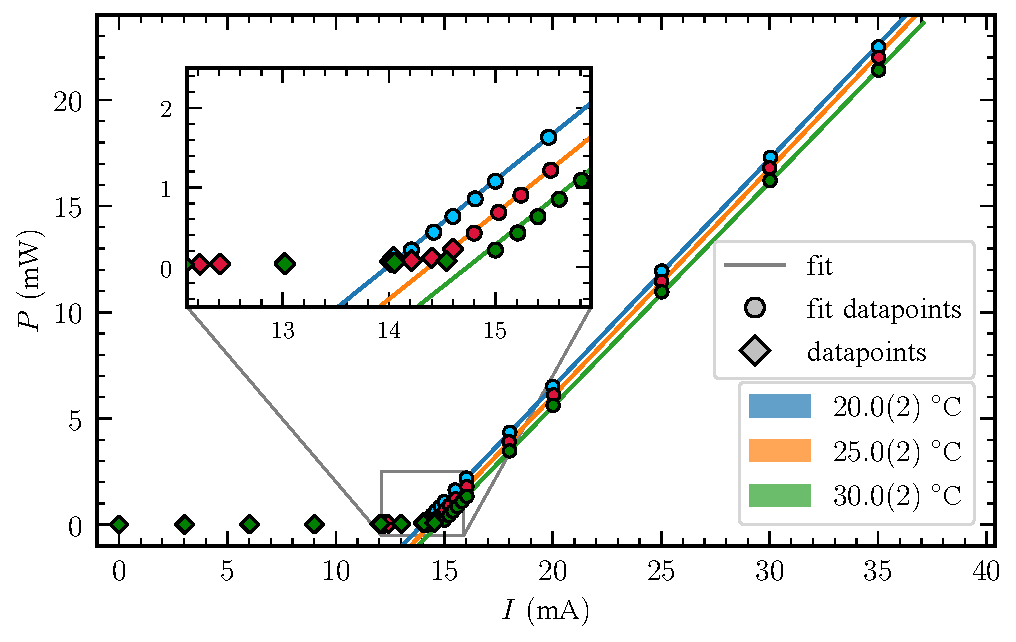
\includegraphics[width=\textwidth]{task1}
	\caption{The output power $P$ of the laser is measured for different currents $I$ and temperatures $T$. Linear functions are fitted to datapoints in the linear regime (circles), while the data not used for fitting are rhombi. The measurements at different temperatures are marked with different colors.}
	\label{fig:power}
\end{figure}

Theory tells us (see \autoref{subsec:diode}), that below a threshold current $I_\mathrm{th}$, the emitted power of the laser comes from spontaneous emission without much increase in power with added current. Above $I_\mathrm{th}$ lasing starts and the power dependence is linear. Looking at \autoref{fig:power} one can clearly see the two regions with $I_\mathrm{th}$ lying around $14 \unit{mA}$. It is also apparent, that $I_\mathrm{th}$ moves to higher currents with increasing temperature. To accurately determine the threshold current and the efficiency of the laser we selected datapoints in the linear region and fitted a linear function of the type $P(I) = \eta (I - I_\mathrm{th})$. The fitted values for threshold current $I_\mathrm{th}$, efficiency $\eta$ and differential quantum efficiency $\eta_d$ can be seen in \autoref{table:eta}.

\begin{center}
	\captionof{table}{Fitted threshold current $I_\mathrm{th}$, efficiency $\eta$ and differential quantum efficiency $\eta_d$ for three different temperatures.\vspace{0.3cm}}
	\begin{tabular}{@{\extracolsep{5mm}} 
			l
			S[table-format=2.3(2)]
			S[table-format=1.3(1)]
			S[table-format=1.4(1)]
		}
		\toprule
		\makecell[t]{\( T \) in \( \oldunit{\degreeCelsius} \)}
		&   {\makecell[t]{\( I_\mathrm{th} \) in \( \unit{mA} \)}}
		&   {\makecell[t]{\( \eta \)}}
		&   {\makecell[t]{\( \eta_d \)}}\\
		\midrule
		\( 20.0(2) \) & 13.982(14) & 1.075(4) & 0.581(2) \\
		\( 25.0(2) \) & 14.374(15) & 1.072(5) & 0.579(3) \\
		\( 30.0(2) \) & 14.73(4) & 1.06(1) & 0.572(5) \\
		\bottomrule
	\end{tabular}
	\label{table:eta}
\end{center}\vspace{0.5cm}
After determining the power characteristics of the laser, the frequency dependence is of importance. To analyze this, we used a setup including a Fabry-Perot interferometer (FPI) and an oscilloscope, as described in \autoref{sec:procedure}. 

In order to analyze frequencies, we need to convert the time domain measurements from the oscilloscope to frequencies. This can be done assuming $\text{FSR}_\text{FPI} = 630 \unit{GHz}$ and using the difference between  adjacent FPI modes as reference length. The differences were calculated by fitting pseudo-voigt functions \autocite{voigt} to isolated and prominent peaks from 10 handpicked datasets. 

The raw data can be seen in \autoref{fig:heatmaps}. Here the frequency spectrum from the oscilloscope is plotted against the laser current, whilst colors represent the voltage amplitude of the recorded spectrum. The heatmaps are labelled according to the value (temperature or current) that remained constant over the measurements.\vspace{0.3cm} 

\begin{figure}[H]
	\centering
	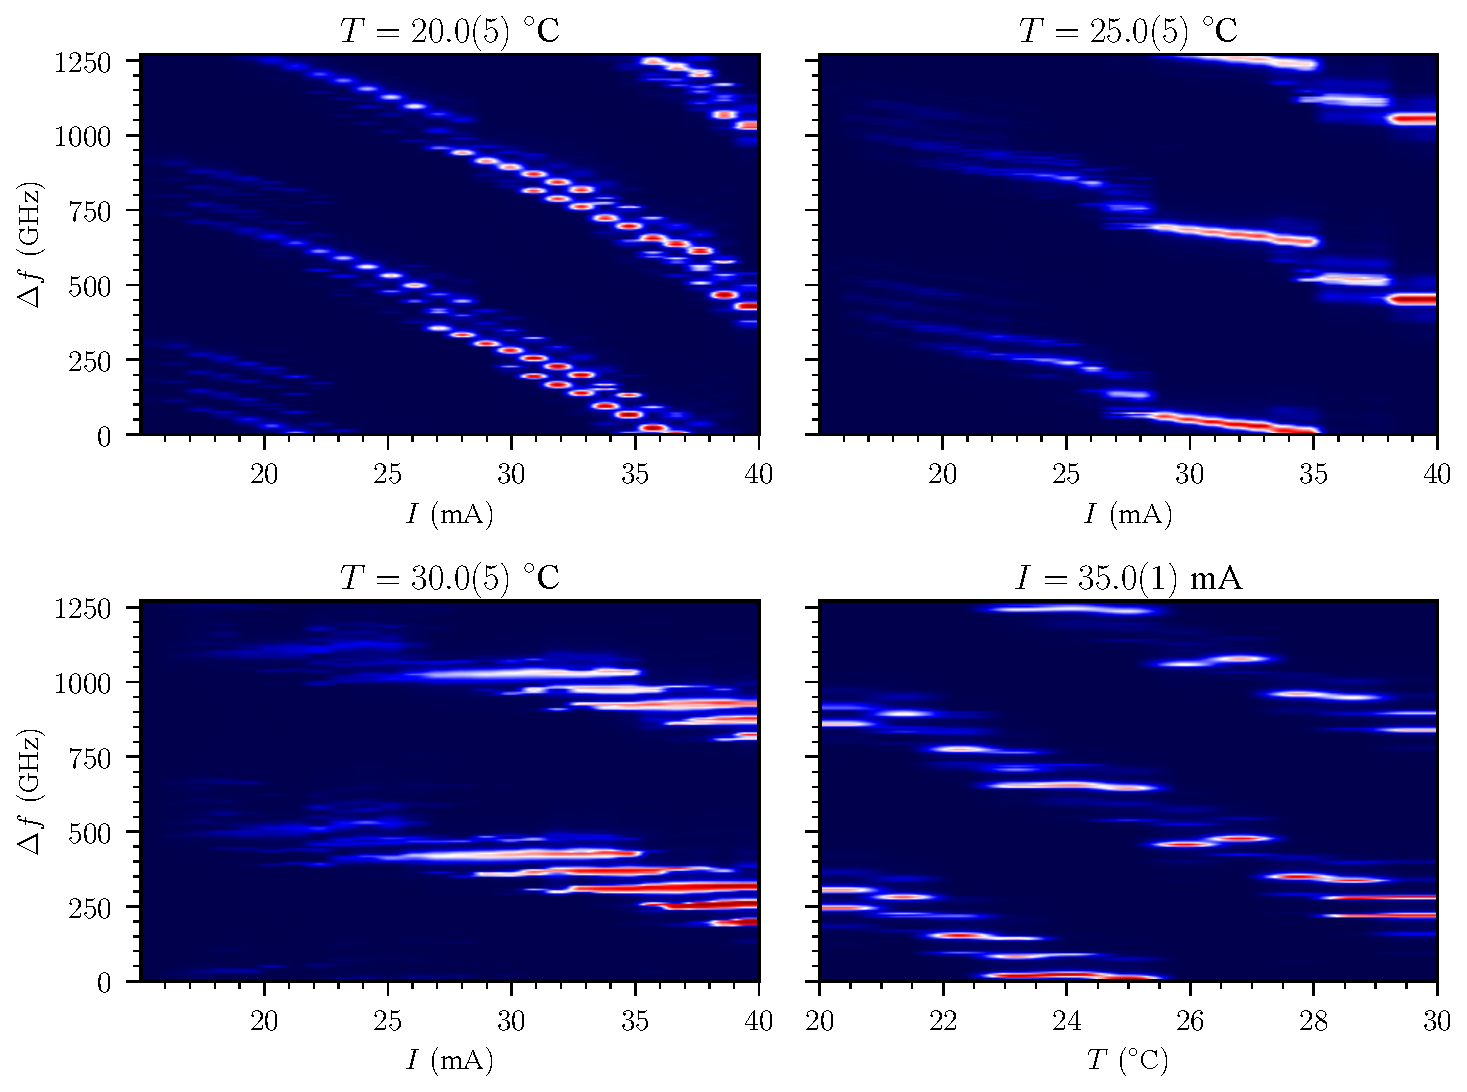
\includegraphics[width=\textwidth]{heatmaps}
	\caption{Heatmaps of the frequency spectrum holding one control parameter (temperature or current) constant and varying the other one. The colors are a proxy for the laser power, represent the amplitude of the signal on the oscilloscope.}
	\label{fig:heatmaps}
\end{figure}

In \autoref{fig:heatmaps} one can clearly see jumps between different lasing modes, as described in \autoref{subsec:modes}. To put numbers on the frequency characteristics of the laser we have to analyze the position and width of the peaks in intensity. We did this by firstly normalizing the data to lie between 0 and 1 using the highest datapoint and then locating peaks that lie above $0.85$, since we can have multiple modes with expressed peaks, depending on the gain profile. This value was manually chosen such that we catch prominent overlapping modes without littering the subsequent plots with less important datapoints (we are mainly interested in the dominant mode). Once we have located the peaks used for analysis, we fit a pseudo-voigt function to data withing $25 \unit{GHz}$ of the peak. From this we can extract the center of the peak, with the full width at half minimum (FWHM) as chosen uncertainty.

In \autoref{fig:fitI} one can see the relative frequency shift of the laser $\Delta f$ with respect to input current $I$, whilst holding the temperature $T$ constant. We chose the first datapoint to be the frequency reference. We identified datapoints belonging to the same mode by overlaying \autoref{fig:fitI} with the heatmaps from \autoref{fig:heatmaps} and grouped the data by color. Data not belonging to any major mode are marked white. Additionally we fitted linear functions of the type $f(I) = kf + d$ to every mode (solid lines) and once to all data (dashed line). Both x- and y-error are almost too small to make out in the plot. 

\begin{figure}[H]
	\centering
	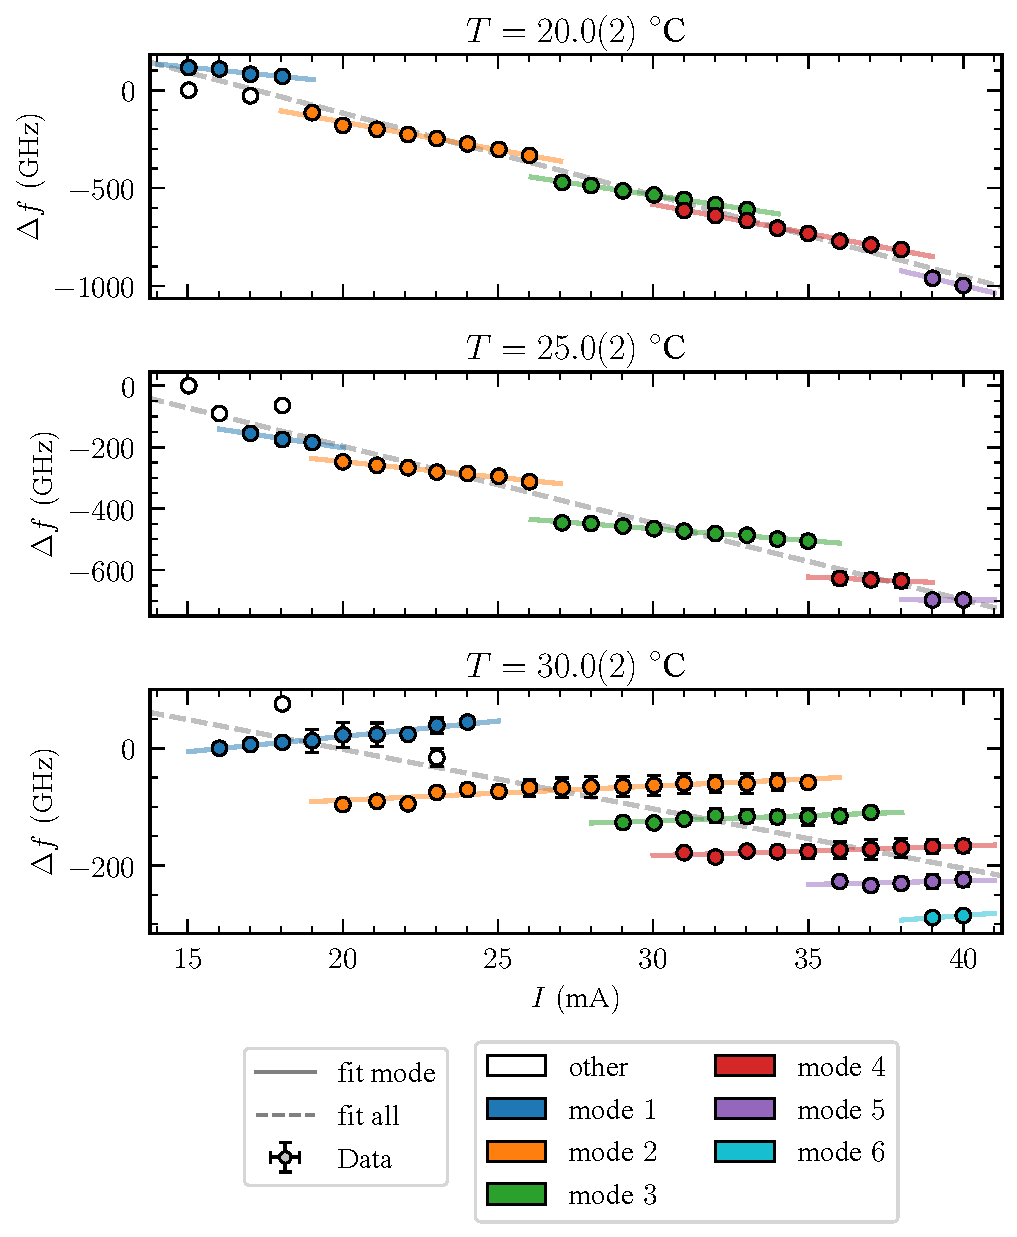
\includegraphics[width=\textwidth]{fitI}
	\caption{The fitted frequency of intensity peaks, relative to the first datapoint, is plotted for three different temperatures and varying current. The temperature can be seen above the plot. Datapoints lying on different modes were identified and marked by color. Linear function were fitted to the different modes (solid lines) and once to the entire data (dashed line).}
	\label{fig:fitI}
\end{figure}

The same was done with swapped control parameters, keeping the current constant at $I~=~35.00(1) \unit{mA}$  and varying the temperature in steps of $1 \unit{\degreeCelsius}$. A finer step size could not be realized due to the coarse scale on the laser. Again, the modes were determined by comparing the data with \autoref{fig:heatmaps}, which is of big importance here, since we only have at  most three datapoints in the same mode.

\begin{figure}[H]
	\centering
	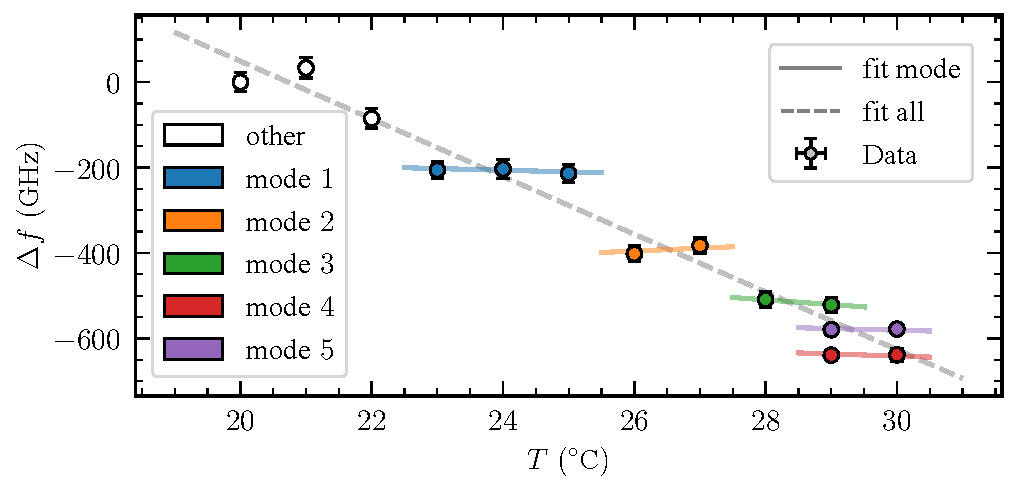
\includegraphics[width=\textwidth]{fitTemp}
	\caption{The fitted frequency of intensity peaks, relative to the first datapoint, is plotted at varying temperatures,  holding current constant at $35.00(1) \unit{mA}$. Datapoints lying on different modes were identified and marked by color. Linear function were fitted to the different modes (solid lines) and once to the entire data (dashed line).}
	\label{fig:fitT}
\end{figure}

The determined slopes from all the linear fits can be found in \autoref{table:Fits}. Since we fitted functions with two free parameters, fits that were performed on few datapoints should be taken with caution. When dealing with only two datapoints, the uncertainty of the slope is omitted in \autoref{table:Fits}, since it can not be defined in a meaningful way.  

\begin{center}
	\captionof{table}{The slopes for all fits seen in \autoref{fig:fitI}. Some values have purposely missing uncertainties, since there are no degrees of freedom left in the fits.\vspace{0.3cm}}
	\begin{tabular}{@{\extracolsep{5mm}} 
			l
			S[table-format=2.1(1)]
			S[table-format=2.1(1)]
			S[table-format=2.1(1)]
			S[table-format=2.1(1)]
			S[table-format=2.1(1)]
			S[table-format=1]
			S[table-format=1]
			S[table-format=2.1(1)]
		}
		\toprule
		& \multicolumn{7}{c}{\makecell{slope of mode fit in $\oldunit{GHz/K}$}} \\
		\cmidrule(lr){2-8}
		{$T$ in $\oldunit{\degreeCelsius}$}
		&   {1}
		&   {2}
		&   {3}
		&   {4}
		&   {5}
		&   {6}
		&   {all}\\
		\midrule
		\( 20.0(2) \) & -16(5) & -28(2) & -24(2) & -30(1) & -37 &  & -41.8(2) \\
		\( 25.0(2) \) & -15(7) & -10(2) & -8(2) & -4(13) & 0 &  & -27.3(4) \\
		\( 30.0(2) \) & 5(1) & 5(1) & 2(1) & 1(1) & 1(3) & 4 & -10.1(2) \\
		\bottomrule\addlinespace[1.5ex]
		& \multicolumn{7}{c}{\makecell{slope of mode fit in $\oldunit{GHz/mA}$}} \\
		\cmidrule(lr){2-8}
		{$I$ in $\oldunit{mA}$}
		&   {1}
		&   {2}
		&   {3}
		&   {4}
		&   {5}
		&   {6}
		&   {all}\\
		\midrule
		\( 35.00(2) \) & -3(6) & 19.2 & -13.0 & 0.8 & 1.4 & & -67.3(6) \\
		\bottomrule
	\end{tabular}
	\label{table:Fits}
\end{center}\vspace{0.5cm}
Lastly, we will determine the free spectral range (FSR) of the diode. For this we need to measure the distance between adjacent peaks from the same FPI mode. As can be seen in \autoref{fig:heatmaps} and \autoref{fig:fitI}, the best data for this  analysis is with constant temperature at $30 \unit{\degreeCelsius}$, since we have multiple peaks at the same current value. Again, we fitted voigt profiles to the peaks and calculated the difference. We get a mean mode spacing of 
$$\text{FSR}_\text{diode} = 62(2) \unit{GHz}.$$ 